\documentclass{standalone}
\usepackage{tikz}

\begin{document}
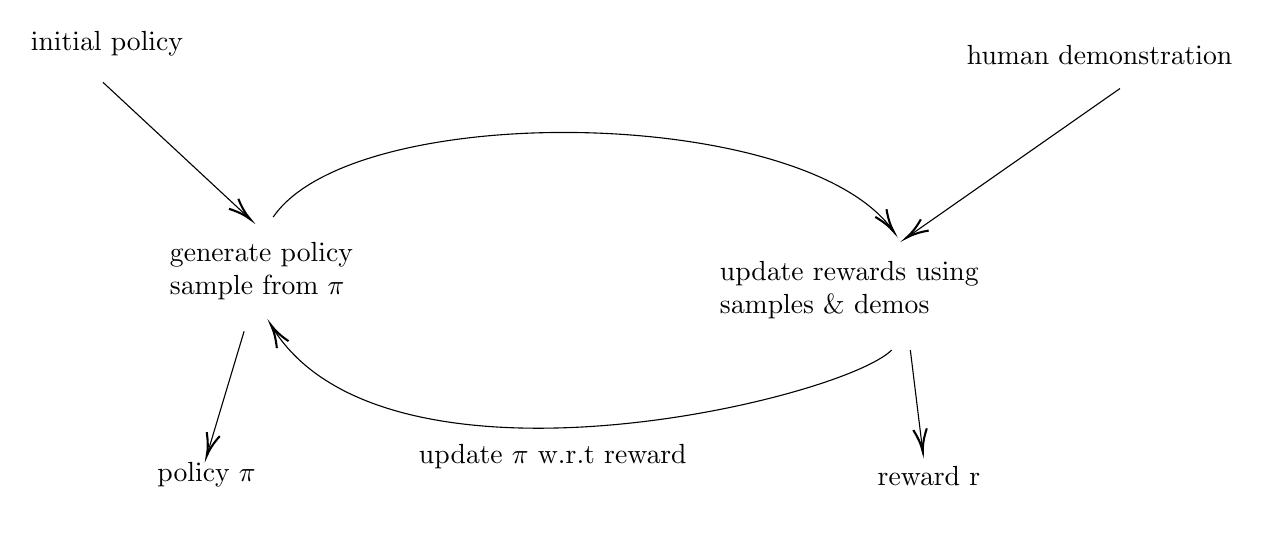
\begin{tikzpicture}[x=0.75pt,y=0.75pt,yscale=-1,xscale=1]
    %uncomment if require: \path (0,300); %set diagram left start at 0, and has height of 300

    %Curve Lines [id:da8696409530197369] 
    \draw    (153,117) .. controls (191.81,60.33) and (407.82,63.02) .. (451.36,123.14) ;
    \draw [shift={(452,124.05)}, rotate = 235.45] [color={rgb, 255:red, 0; green, 0; blue, 0 }  ][line width=0.75]    (10.93,-3.29) .. controls (6.95,-1.4) and (3.31,-0.3) .. (0,0) .. controls (3.31,0.3) and (6.95,1.4) .. (10.93,3.29)   ;
    %Straight Lines [id:da35687342305070713] 
    \draw    (561,55.05) -- (459.64,125.9) ;
    \draw [shift={(458,127.05)}, rotate = 325.05] [color={rgb, 255:red, 0; green, 0; blue, 0 }  ][line width=0.75]    (10.93,-3.29) .. controls (6.95,-1.4) and (3.31,-0.3) .. (0,0) .. controls (3.31,0.3) and (6.95,1.4) .. (10.93,3.29)   ;
    %Straight Lines [id:da2756139774765858] 
    \draw    (71,52.05) -- (140.54,116.69) ;
    \draw [shift={(142,118.05)}, rotate = 222.91] [color={rgb, 255:red, 0; green, 0; blue, 0 }  ][line width=0.75]    (10.93,-3.29) .. controls (6.95,-1.4) and (3.31,-0.3) .. (0,0) .. controls (3.31,0.3) and (6.95,1.4) .. (10.93,3.29)   ;
    %Curve Lines [id:da41719283741377877] 
    \draw    (451,181.05) .. controls (427.12,204.93) and (207.22,257.52) .. (152.81,170.37) ;
    \draw [shift={(152,169.05)}, rotate = 59.23] [color={rgb, 255:red, 0; green, 0; blue, 0 }  ][line width=0.75]    (10.93,-3.29) .. controls (6.95,-1.4) and (3.31,-0.3) .. (0,0) .. controls (3.31,0.3) and (6.95,1.4) .. (10.93,3.29)   ;
    %Straight Lines [id:da8560493927316521] 
    \draw    (460,181.05) -- (465.76,228.06) ;
    \draw [shift={(466,230.05)}, rotate = 263.02] [color={rgb, 255:red, 0; green, 0; blue, 0 }  ][line width=0.75]    (10.93,-3.29) .. controls (6.95,-1.4) and (3.31,-0.3) .. (0,0) .. controls (3.31,0.3) and (6.95,1.4) .. (10.93,3.29)   ;
    %Straight Lines [id:da4205509832997729] 
    \draw    (139,172.05) -- (121.57,230.13) ;
    \draw [shift={(121,232.05)}, rotate = 286.7] [color={rgb, 255:red, 0; green, 0; blue, 0 }  ][line width=0.75]    (10.93,-3.29) .. controls (6.95,-1.4) and (3.31,-0.3) .. (0,0) .. controls (3.31,0.3) and (6.95,1.4) .. (10.93,3.29)   ;

    % Text Node
    \draw (102,128) node [anchor=north west][inner sep=0.75pt]   [align=left] {generate policy\\sample from $\displaystyle \pi $};
    % Text Node
    \draw (367,137) node [anchor=north west][inner sep=0.75pt]   [align=left] {update rewards using\\samples \& demos};
    % Text Node
    \draw (222,225) node [anchor=north west][inner sep=0.75pt]   [align=left] {update $\displaystyle \pi $ w.r.t reward};
    % Text Node
    \draw (486,33) node [anchor=north west][inner sep=0.75pt]   [align=left] {human demonstration};
    % Text Node
    \draw (35,26) node [anchor=north west][inner sep=0.75pt]   [align=left] {initial policy};
    % Text Node
    \draw (443,236) node [anchor=north west][inner sep=0.75pt]   [align=left] {reward r};
    % Text Node
    \draw (96,234) node [anchor=north west][inner sep=0.75pt]   [align=left] {policy $\displaystyle \pi $};


\end{tikzpicture}
\end{document}

% \tikzset{every picture/.style={line width=0.75pt}} %set default line width to 0.75pt        

